\chapter{Introduction}

One of the most basic and yet often overlooked problems in natural language processing (NLP) is word boundary detection, or tokenization. Identifying words is a critical preprocessing step before almost any other work can be done with text: frequency counting, part-of-speech tagging, parsing, etc.
In many languages, this is far from trivial. The standard orthographies for languages as diverse as Ancient Greek and Latin, and modern languages like Thai, Japanese, and Chinese, lack spaces or any other explicit indicator of word boundaries. (Examples of the standard orthographies for Thai and Japanese are shown in Figures \ref{thaitext} and \ref{jpntext}.) This often results in ambiguity about the proper grouping of characters into words, and difficulty in identifying the boundaries of unknown words.

\begin{figure}
	\begin{center}
		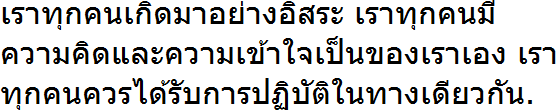
\includegraphics[width=0.75\linewidth]{introduction/udhr_thai}
		\caption[Example of Thai Text]{Example of Thai text. Thai uses spaces to separate clauses, but not individual words \cite{omnithai}.}
		\label{thaitext}
	\end{center}
\end{figure}

\begin{figure}
	\begin{center}
		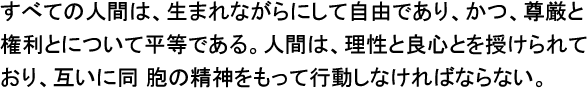
\includegraphics[width=0.75\linewidth]{introduction/udhr_japanese}
		\caption[Example of Japanese Text]{Example of Japanese text. While punctuation and changes in writing system provide some clues, Japanese does not use spaces to separate words or clauses \cite{omnijpn}.}
		\label{jpntext}
	\end{center}
\end{figure}

Substantial research has been done in text segmentation for languages like Chinese and Japanese. The highest-performing systems all use a hybrid approach, incorporating both statistical knowledge to predict probable word boundaries, and access to lexicons to identify known words. Unfortunately, the specific algorithms used are often drastically different, and bespoke tokenizers are typically built on a language-by-language basis. There is no standard, generic framework for handling tokenization across multiple languages. Even in English and other languages that use whitespace in writing, there are numerous edge-cases, such as clitic and punctuation separation, which must be handled with special rules on a per-language basis. In developing software for searching, analyzing, or teaching multiple languages, or supporting natural-language based user interfaces, the complexity of developing separate systems to support equal levels of computer-enhanced interactivity for every desired language quickly becomes impractical. This severely limits both the number of languages that can be supported in any given application and the level of functionality available for each language. Given that the human ability to successfully read any natural language provides an existence proof that a generalized segmentation system (as implemented in the human mind) is possible, it is reasonable to investigate the feasibility of a language-agnostic segmentation system that could be easily integrated into larger natural language processing systems.

In order to make NLP applications more accessible in a wider variety of languages, I am developing a generalizable framework for tokenization which can be easily adapted to any given language. The general tokenization problem can be broken down into a few generic parts, regardless of the language involved: a hypothesis generator, which makes use of both a morphological recognizer encoding lexical knowledge and a statistical model or models, and a selector, which identifies the best hypothesis. Even if a single master system cannot be used for every language, decomposing the problem in this way should allow for replacing only certain parts and reusing others, as long as the replacement modules conform to a standard interface.

For the purposes of this thesis, I have focused only on the hypothesis generation stage. I identify promising lexical (morphological) and statistical models and several methods of integrating them into a single framework for hypothesis generation across multiple languages. I then test these systems on corpora of native-speaker texts from three typologically dissimilar languages. The success of each system is determined by two major factors. The first is generalizability, or the consistency of results across multiple languages. Generalizability, however, is a necessary but not sufficient condition for a generic tokenization framework. The second factor is token-recognition performance. Additionally, hybrid systems can be evaluated in terms of their improvement over morphological or statistical methods used alone. I show that a hybrid system based on this framework:

\begin{enumerate}
\item does generalize well across a variety of languages,
\item produces results comparable to those of state-of-the-art
tokenization systems developed for specific languages, and
\item outperforms both morphological and statistical methods used individually.
\end{enumerate}